\begin{floatingfigure}{2.8in}
\vspace{-0.1in}
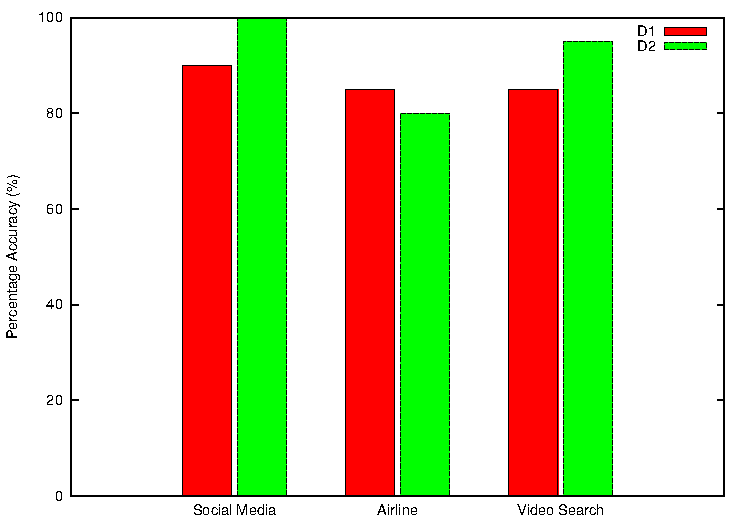
\includegraphics[scale=.45]{dev_results}
\vspace{-0.08in}
\caption{Porting effort analysis accuracy\label{fig:dev_results}}
\end{floatingfigure}

I started this research with a comprehensive study on machine-readable 
API description languages. This initial survey lead me to develop a formal 
mechanism for automatically estimating the application porting effort between 
different APIs and API versions~\cite{6930607}. My algorithm takes two API descriptions 
(source API and target API) as the input, which contain axiomatic semantics~\cite{Hoare:1969:ABC:363235.363259} of 
API operations expressed in a Python-based syntax, and calculates a numeric 
value that is indicative of the effort that would be required in porting an application 
from the source API to the target API. This formal approach makes use of Dice 
coefficient~\cite{dice1945,738528} to quantify the similarity between axiomatic semantic predicates of APIs, 
and also makes use of Hoare's consequence rules~\cite{Hoare:1969:ABC:363235.363259}. The overall method has been 
validated against both randomly generated and real world API descriptions. 
I also combined my approach with k-means clustering in order to classify API pairs into 
multiple categories (typically 2 -- easy and hard) based on the relative difficulty in 
porting applications between them. Developer studies have shown that my 
automated mechanism closely resembles the relative difficulty 
that human programmers associate with porting applications across web APIs.
Figure~\ref{fig:dev_results} shows the percentage accuracy of the automated API
classification, with respect to the manual classifications by two human programmers
(D1, D2), applied on three real world API collections.

Recently, I have further extended my automated porting effort calculation 
mechanism to also take the syntactic features of web APIs into consideration. This 
results in a two-phase API comparison algorithm where the first phase performs a 
syntactic comparison between APIs (i.e operations, input/output types), and the 
second phase performs the semantic analysis described earlier. The syntactic 
comparison is based on well-established programming languages research and 
static type checking methods.

\begin{figure}
\centering
\begin{subfigure}{.5\textwidth}
  \centering
  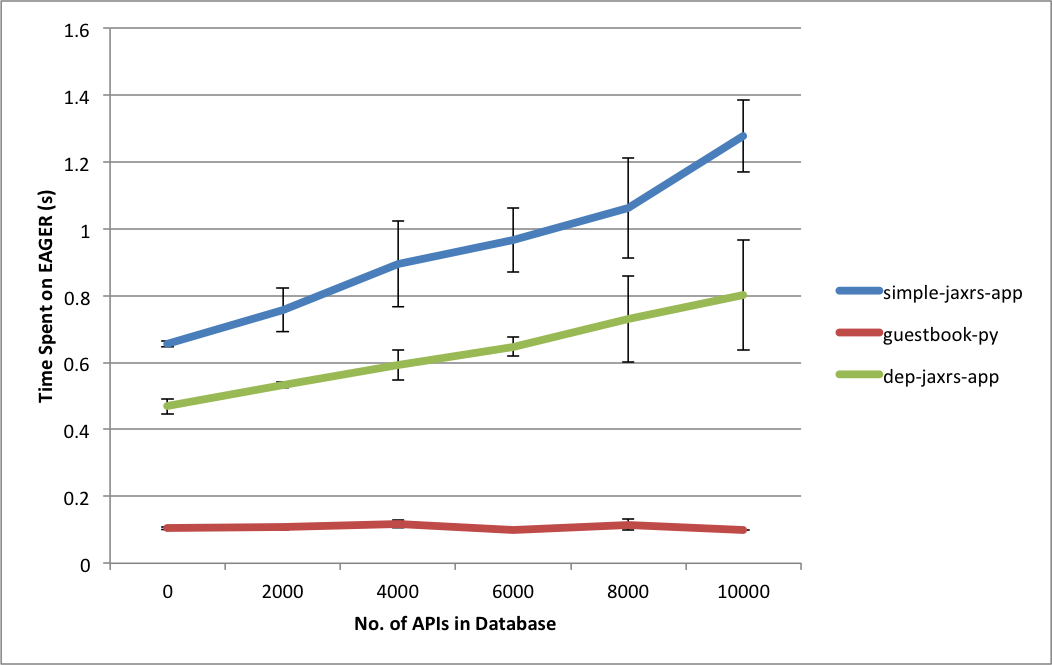
\includegraphics[width=.75\linewidth]{scalability}
  \caption{Overhead vs. number of APIs}
  \label{fig:sub1}
\end{subfigure}%
\begin{subfigure}{.5\textwidth}
  \centering
  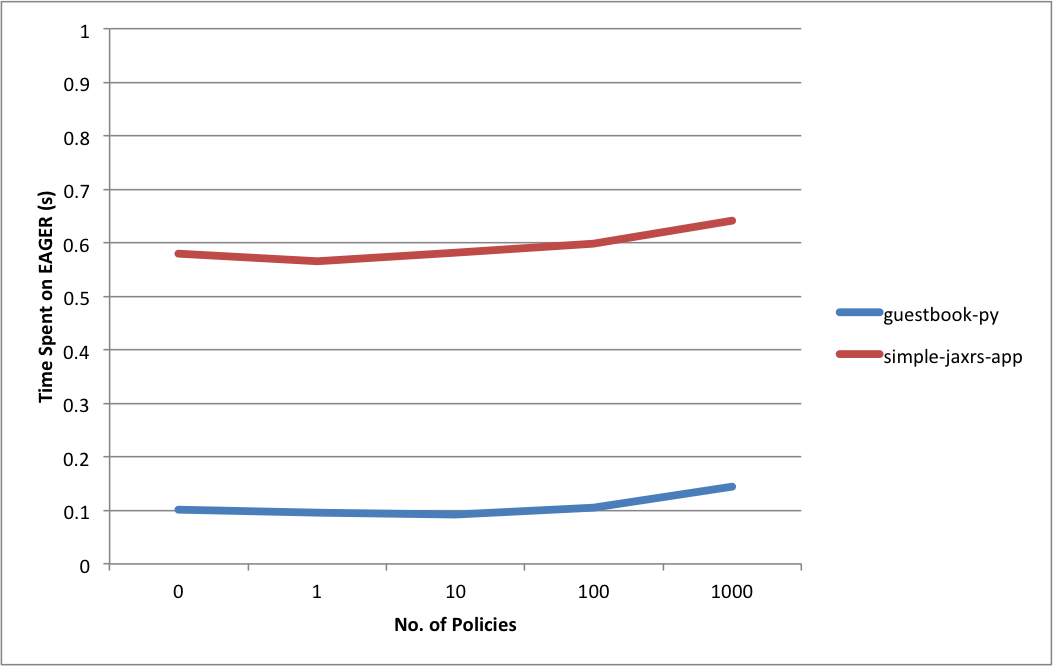
\includegraphics[width=.75\linewidth]{overhead_by_policies}
  \caption{Overhead vs. number of policies}
  \label{fig:sub2}
\end{subfigure}
\caption{EAGER performance overhead and scaling patterns}
\label{fig:eager_perf}
\end{figure}

In an effort to support design-time API governance as a cloud-native feature in 
modern clouds, I designed EAGER (Enforced API Governance Engine for REST), a 
system that augments PaaS clouds~\cite{6903538}. EAGER intercepts all application and API 
deployment requests issued by developers, and validates them against a set of 
admin-specified policies. Application and API metadata are further subjected to a wide 
range of built-in sanity checks, which include an API backwards-compatibility test based 
on the syntactic comparison method described earlier. Applications and APIs are only 
hosted in the cloud, if all the policy and sanity checks return successfully. We used a 
restricted subset of Python as the policy specification language, which allows programmers 
to write powerful governance policies in a very simple and intuitive way. EAGER's policy engine 
prevents all I/O operations, most third party library calls, and also global in-memory state, in 
order to perform policy validations in a stateless and side-effect free manner. EAGER also 
supports dependency management, OAuth based authorization for all deployed APIs and does 
not require any major changes to the existing cloud architecture. I implemented an EAGER 
prototype using the AppScale~\cite{krintzappscale13} open source PaaS (open source Google App Engine clone), 
and demonstrated that EAGER adds negligible overhead to the typical application deployment 
process in the cloud and it scales to handle thousands of APIs and policies. Figure~\ref{fig:eager_perf}
shows how the EAGER overhead varies for different example web applications, under different
conditions.

Currently I'm conducting research in the area of automated performance analysis of web
services at development time (i.e. before services are deployed into the cloud). I'm using
prominent static analysis methods (abstract interpretation based loop bound analysis,
branch prediction, WCET analysis etc.~\cite{ermedahl_et_al:OASIcs:2007:1194,Yeh:1991:TAT:123465.123475,bygde2010static}) 
to compute paths of execution through service 
implementations. I use this information to build profiles of services which
specify what core cloud services and APIs are being used in a service implementation,
and in which order and frequency. My goal is to combine this information with historical
performance data of the APIs, using simulation methods or other non-parametric statistical
methods~\cite{Nurmi:2007:QQB:1791551.1791556} and derive bounds on the performance expected from the services with high
certainty. 
Such information can be used to formulate SLAs for the services or tune
the service implementations for better performance. 
I have already conducted some preliminary tests in this area using real world
Java web applications developed for the Google App Engine (and AppScale) environment,
and the initial results are quite encouraging.
In the future I intend to further extend 
these methods to perform SLA management and enforcement at runtime.